\documentclass[10pt]{article}
\usepackage[utf8]{inputenc}
\usepackage{graphicx}
\usepackage{amsmath}
\usepackage{amssymb}
\usepackage{geometry}
\usepackage{setspace}
\usepackage{abstract}
\usepackage{titlesec}
\usepackage[backend=biber,style=apa]{biblatex}% Changed style to apa
\usepackage[hidelinks]{hyperref}
\PassOptionsToPackage{hyphens}{url} % Pass hyphens option to url package via hyperref
\usepackage{fancyhdr} % For custom headers and footers
\usepackage{lastpage} % For page numbering in the footer
\usepackage{xcolor} % For text color
\usepackage{tabularx} % Tabularx package for better table formatting
\usepackage{longtable}% Long table package for tables that span multiple pages

% Set marginparwidth for todonotes
\setlength{\marginparwidth}{2cm} % Adjust the marginparwidth
\usepackage{todonotes} % TODOs
\usepackage{tcolorbox} % For colored boxes
\usepackage{caption} % For custom captions

% Fonts and typography
\usepackage{helvet} % Load the Helvetica font package
\renewcommand{\familydefault}{\sfdefault} % Set sans-serif as the default font family

% Page setup
\geometry{margin=1in}
\setstretch{1.2}
\titleformat{\section}{\bfseries\Large}{\thesection}{1em}{}
\titleformat{\subsection}{\bfseries\large}{\thesubsection}{1em}{}
\titleformat{\subsubsection}{\bfseries\normalsize}{\thesubsubsection}{1em}{}

% Add bibliography file
\addbibresource{references.bib}

% Customization to remove url date and format URLs and DOIs
\AtEveryBibitem{%
  \ifentrytype{online}{%
    \clearfield{urldate}%
    \clearfield{note}%
  }{}%
  \ifentrytype{article}{%
    \clearfield{urldate}%
  }{}%
}

\renewbibmacro*{doi+eprint+url}{%
  \printfield{doi}%
  \newunit\newblock%
  \iffieldundef{doi}{%
    \usebibmacro{eprint}%
    \newunit\newblock%
    \usebibmacro{url+urldate}}%
    {}%
}

% Customize the caption format
\captionsetup[figure]{
    labelfont=bf,           % Bold font for the label
    labelsep=space           % Use a space as the separator
}
% \captionsetup[table]{
%     labelfont=bf,           % Bold font for the label
%     labelsep=space           % Use a space as the separator
% }

% Change font size of bibliography entries
\renewcommand{\bibfont}{\fontsize{7pt}{9pt}\selectfont}% Set font size to 7pt, maybe too small. Change to 8pt if needed. Also adjust actual text size?

% Title
\title{Visual Cortical Prostheses: Bridging Technology, AI and Human Vision for the Future}
\author{
  Marc J. Posthuma\\
  Student Number: 4413105\\
  \texttt{marc.posthuma@ru.nl}\\
  \\
  Radboud University\\
  Supervisor: dr.\ F.\ Zeldenrust\\
  Department of Neurophysics, Donders Centre for Neuroscience
}
\date{\today}

% Adjust page geometry to balance header and footer
\geometry{
  a4paper,
  left=20mm,
  right=20mm,
  top=30mm,
  bottom=30mm,
  headheight=60.50554pt, % Set the head height
  headsep=10pt, % Space between header and text
  footskip=30pt % Space between text and footer
}

% Custom footrule commands
\newcommand{\blackfootrule}{%
  \color{black}\makebox[\headwidth]{\rule[0.5ex]{\headwidth}{0.3pt}}%
}

\newcommand{\grayfootrule}{%
  \color{gray}\makebox[\headwidth]{\rule[0.5ex]{\headwidth}{0.3pt}}%
}

% Define fancyhdr styles
\fancypagestyle{firstpage}{
  \fancyhf{}
  \fancyhead[L]{
\includegraphics[width=5cm, keepaspectratio]{imgs/RU_logo_NL_cropped.png}}
  \fancyhead[R]{\fontsize{10}{12}\selectfont \textbf{Research Proposal} \\ NWI-BM-RESPROP}
  \fancyfoot[L]{\fontsize{8}{10}\selectfont \textcolor{gray}{Radboud University}}
  \fancyfoot[C]{\fontsize{8}{10}\selectfont \textcolor{gray}{\thepage\ of~\pageref{LastPage}}}
  \fancyfoot[R]{\fontsize{8}{10}\selectfont \textcolor{gray}{July 2024}}
  \renewcommand{\footrulewidth}{0.3pt}
  \renewcommand{\footrule}{\blackfootrule}
}

\fancypagestyle{rest}{
  \fancyhf{}
  \fancyhead[L]{\fontsize{8}{10}\selectfont \textcolor{gray}{Research Proposal}}
  \fancyhead[R]{\fontsize{8}{10}\selectfont \textcolor{gray}{Visual Cortical Prostheses: Bridging Technology, AI and Human Vision for the Future}}
  \fancyfoot[L]{\fontsize{8}{10}\selectfont \textcolor{gray}{Radboud University}}
  \fancyfoot[C]{\fontsize{8}{10}\selectfont \textcolor{gray}{\thepage\ of~\pageref{LastPage}}}
  \fancyfoot[R]{\fontsize{8}{10}\selectfont \textcolor{gray}{July 2024}}
  \renewcommand{\footrulewidth}{0.3pt}
  \renewcommand{\footrule}{\grayfootrule}
}

% Redefine the abstract environment to use "Summary" instead of "Abstract"
\makeatletter
\renewenvironment{abstract}{%
    \if@twocolumn%
      \section*{\abstractname}%
    \else
      \begin{center}%
        {\bfseries \large\abstractname\vspace{-.5em}\vspace{\z@}}%
      \end{center}%
      \quotation\small % Ensures the text is smaller
    \fi}
    {\if@twocolumn\else\endquotation\fi}%
\renewcommand{\abstractname}{Summary}
\makeatother

% Document
\begin{document}

% \pagestyle{plain}% Default plain page style for the list of TODOs
% \listoftodos% Remove this line before submission
% \clearpage%To make sure the todo list is on a separate page without fancyhdr

% \newpage% To make sure the todo list is on a separate page without fancyhdr

% Title and abstract
\maketitle
\thispagestyle{firstpage} % Apply first page style after title
\begin{abstract}
  \noindent Visual cortical prostheses represent a revolutionary technology
  within the field of neuroprosthetics, aimed at restoring vision for
  individuals with visual impairments through direct neural interfaces. Recent
  advances have focused on retinal and optic nerve implants; however, these do
  not aid individuals with damage beyond these structures. This proposal
  explores the use of artificial intelligence (AI) and virtual reality (VR) to
  optimize visual cortical prostheses by developing AI algorithms that generate
  and refine phosphene patterns, enabling users to visualize dynamic
  environments in real-time. Expanding upon existing phosphene simulators that
  are limited to static images, this research aims to enhance scene
  simplification, phosphene resolution, and the dynamic temporal aspects of
  phosphenes, improving the quality and accuracy of visual representations.

  The research is divided into three phases. The first phase involves developing
  initial AI algorithms for scene simplification and phosphene generation using
  Convolutional Neural Networks (CNNs), alongside setting up the experimental
  infrastructure. Diverse groups of 20 participants with normal and impaired
  vision will navigate VR environments to collect data on the effectiveness of
  these algorithms. The second phase advances AI models using CNNs, Generative
  Adversarial Networks (GANs), and Reinforcement Learning (RL), coupled with
  neurophysiological studies such as Visual Evoked Potentials (VEP) and fNIRS to
  assess the impact on visual perception. These advanced models will focus on
  capturing and optimizing the dynamic temporal characteristics of phosphenes,
  ensuring that the visual information remains coherent and accurate over time.
  The final phase conducts extensive experiments with a larger participant group
  to validate the AI systems, aiming for real-world application readiness.

  This study aims to significantly enhance the user experience of visual
  prosthetics, potentially transforming the field by enabling accurate, dynamic
  visual representations via the use of advanced AI solutions. If successful, it
  will pave the way for advanced neural interfaces and sensory augmentation
  devices, improving the quality of life for individuals with visual impairments.
  The research highlights the importance of interdisciplinary collaboration in
  advancing neuroprosthetic technology, urging continued innovation at the
  intersection of neuroscience, engineering, and AI\@.
\end{abstract}
\textbf{Keywords:} Simulated  phosphene vision, neuroprosthetics, deep learning models, phosphene patterns, real-time image processing

\pagestyle{rest} % Apply rest page style from here
\clearpage % Ensure a new page for the figure and introduction

\begin{figure*}[ht!]
  \centering
  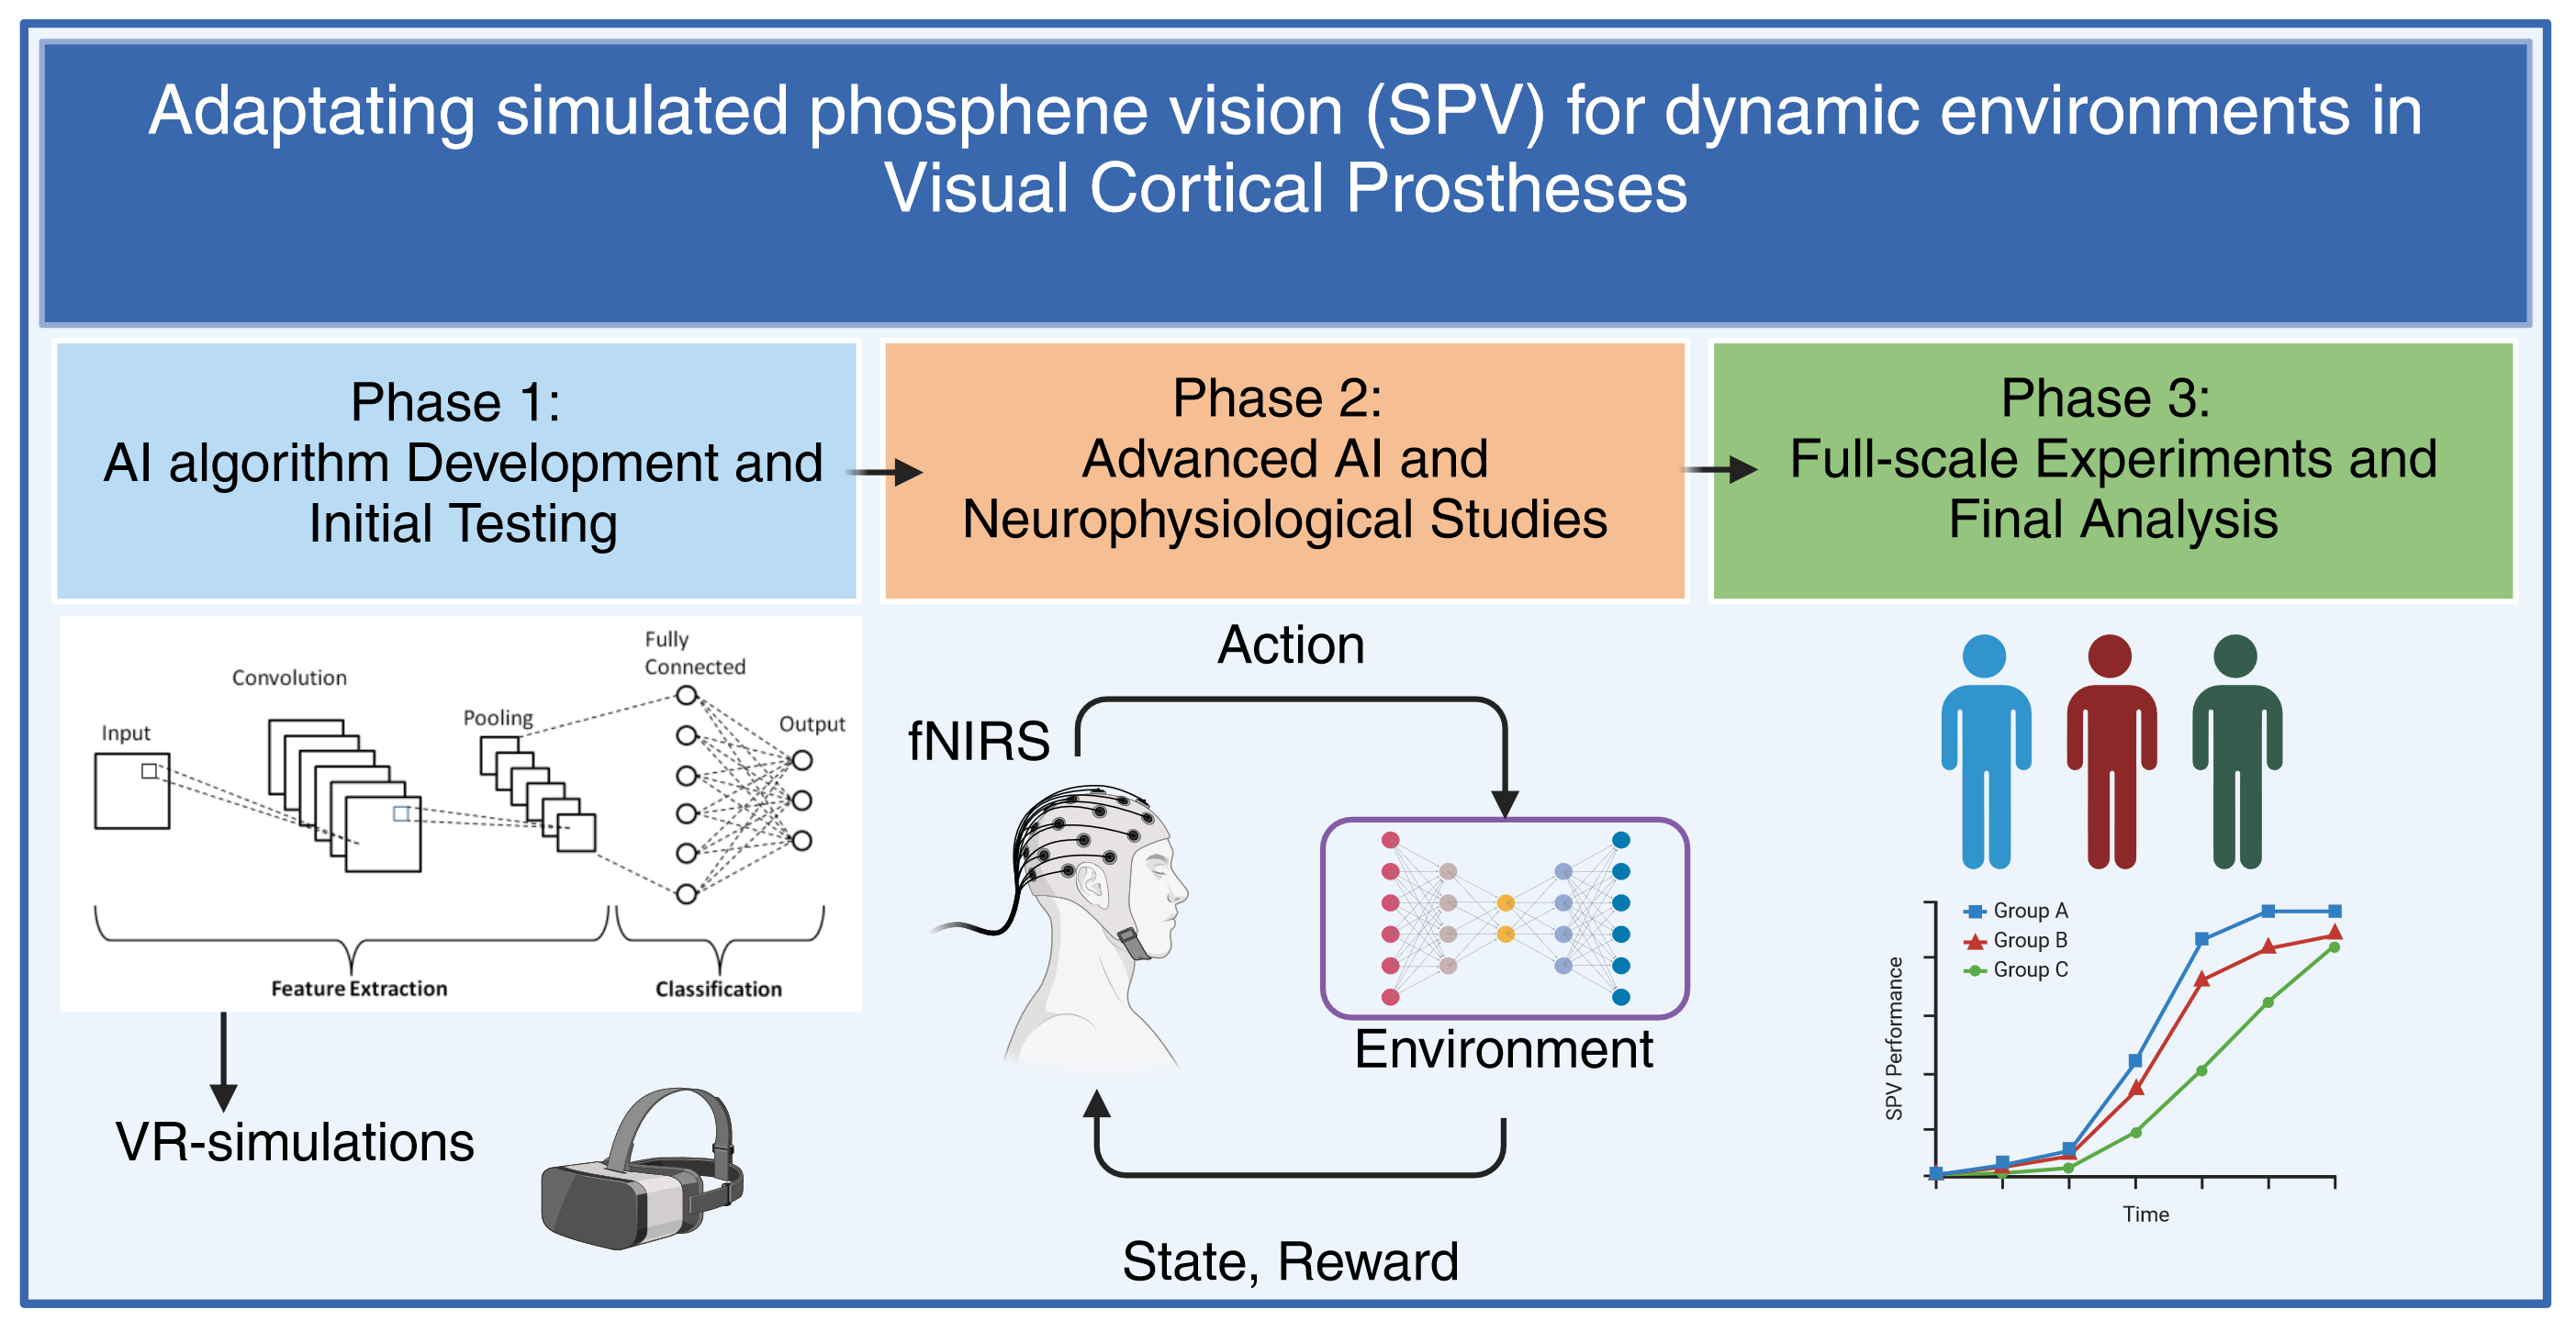
\includegraphics[width=1.0\textwidth]{imgs/SPV_VCP_pipeline.png}
  \caption{| Graphical abstract illustrating the three phases of the research proposal on simulated phosphene vision for visual cortical prostheses: (1) Developing initial AI algorithms for scene simplification and phosphene generation; (2) Advancing AI models with neurophysiological assessments; (3) Conducting extensive experiments for real-world application validation. (Image: BioRender, \href{https://app.biorender.com/}{https://app.biorender.com/}, accessed on 2 July 2024).}\label{fig:graphical_abstract}
\end{figure*}

\section*{Introduction}\label{sec:intro}
\subsection*{Background}\label{subsec:background}
Globally, blindness affects millions of people, with estimates rising from over
30 million in 2013 to 43.3 million in
2020~\parencite{stevensGlobalPrevalenceVision2013,bourneTrendsPrevalenceBlindness2021}.
For certain types of blindness, visual prosthetics present a promising avenue
for restoring rudimentary vision through electrical stimulation of the visual
system. In the past decade, significant attempts have already been made in early
systems that focus on retinal and optic nerve implants, such as the exemplary
FDA-approved ARGUS-II retinal system by Second Sight
Medical~\parencite{hoLongTermResultsEpiretinal2015}. However, these systems do
not provide a solution for individuals who have damage to structures such as the
retina or optic nerve in the visual pathway.

Visual cortical prostheses provide a novel approach to stimulating the brain by
interface directly with the brain's visual
cortex (Figure~\ref{fig:schematic}).
These devices convert visual information from the environment into neural
signals that can be processed by the brain.

The core technology involves the generation of phosphenes—perceived spots of
light resulting from electrical stimulation of the visual
cortex~\parencite{vandergrintenBiologicallyPlausiblePhosphene2024}. However,
organizing these phosphenes into coherent and interpretable visual patterns
remains a significant challenge.

\begin{figure*}[ht!]
  \centering
  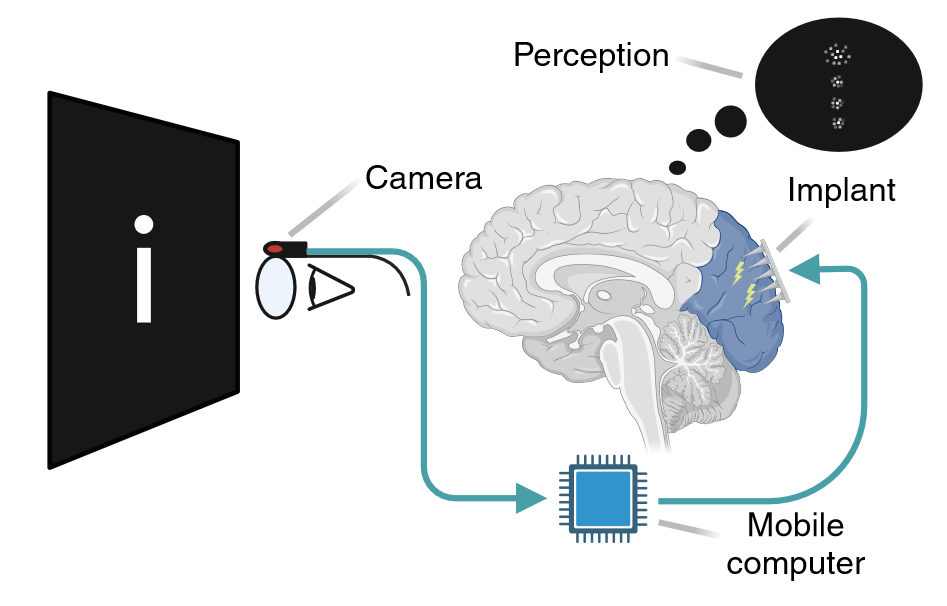
\includegraphics[width=0.7\textwidth]{imgs/visual_cortical_prothesis.png}
  \caption{| Functional schematic representation of a visual cortical
    prosthesis. The visual environment is recorded by a wearable camera
    and sent to a (wireless) mobile computer. Electrodes within a brain
    implant are then selectively activated to stimulate neurons in the
    primary visual cortex (V1). By leveraging the retinotopic
    organization of V1, a precise pattern of phosphenes is created,
    forming a coherent representation of the visual
    scene~\parencite{chenShapePerceptionHighchannelcount2020}. (Image:
    BioRender,
    \href{https://app.biorender.com/}{https://app.biorender.com/},
    accessed on 27 May 2024).}\label{fig:schematic}
\end{figure*}

In order to optimize these phosphene patterns for more accurate representations
of a user's surroundings, artificial intelligence (AI) can be leveraged in the
form of deep learning algorithms. Algorithms such as Convolutional Neural
Networks (CNNs) have already been proven to be effective for image processing of
static objects in recent work
by~\textcite{deruytervansteveninckEndtoendOptimizationProsthetic2022}. Deep
learning models like CNNs provide a solution to low sampling resolution of
complex visual stimuli, enabling the generation of more detailed and accurate
reconstruction of the visual scene.

The phosphene simulator described in the article
by~\textcite{deruytervansteveninckEndtoendOptimizationProsthetic2022} was
implemented in Python, utilizing the PyTorch deep learning library for its
computational capabilities. It operates by translating electrical stimulation
parameters into an estimated phosphene perception, taking into account the
history of stimulation to ensure accuracy. The simulator initializes with
electrode locations on a flattened cortical map of the primary visual cortex
(V1), using the reverse wedge-dipole visuotopic model to map these locations to
the user's visual field~\parencite{liWearableComputerVision2013}. This model
accounts for the eccentricity and azimuth in the visual field, controlling
various parameters to ensure realistic proportions in cortical distance.

To determine the size of the phosphenes, the simulator uses models that estimate
current spread from the electrodes, incorporating factors like stimulation
current and cortical magnification. The appearance and brightness of phosphenes
are modeled with a sigmoidal activation function, taking into account the
activation threshold, which introduces variability between electrodes. Temporal
dynamics are managed through a memory trace that adjusts phosphene brightness
based on stimulation history, incorporating decay and input effects to simulate
accommodation. Each frame, the simulator processes stimulation parameters,
estimates phosphene characteristics, and renders these effects on a visual field
map, summing them to produce the final simulated prosthetic percept. This
biologically grounded model aims to enhance the realism and efficacy of
simulated prosthetic vision, facilitating the optimization of cortical visual
prosthetic systems. An example of such a framework is shown in Figure~\ref{fig:simulator_framework}.

\begin{figure*}[ht!]
  \centering
  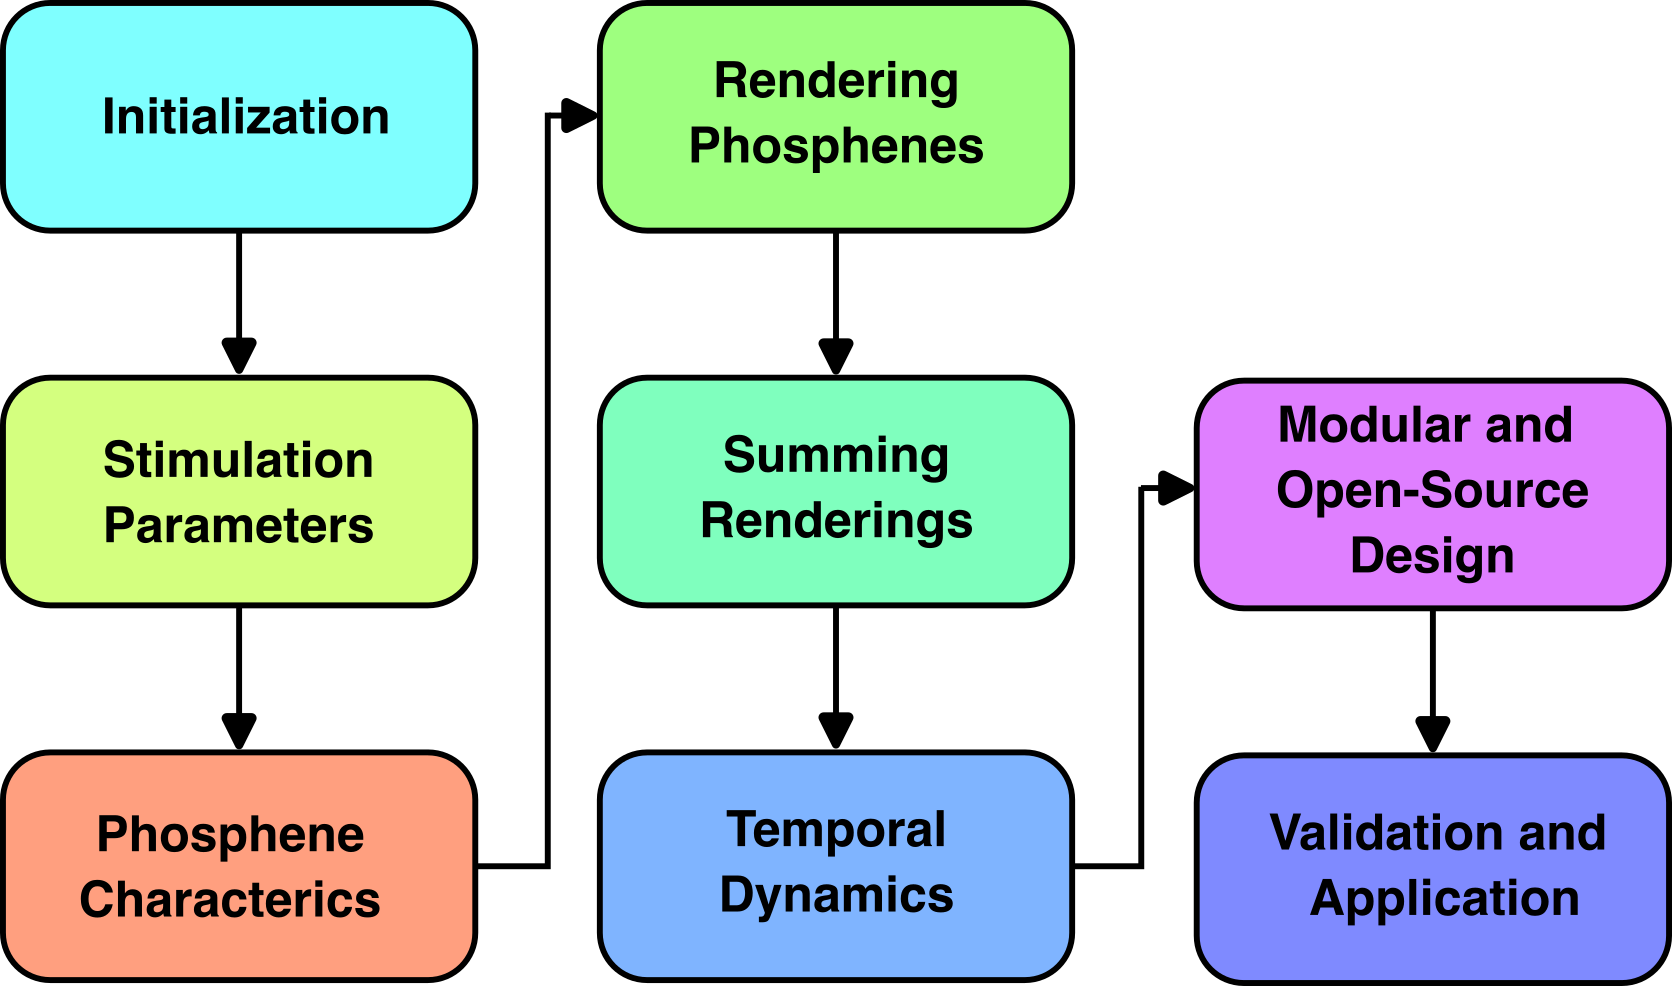
\includegraphics[width=0.6\textwidth]{imgs/block_diagram_vis_prost.png}
  \caption{| Overview of a Visual Prosthesis Simulation Framework. The
    simulator is initialized with electrode locations on a visuotopic map of the
    visual cortex (V1), representing the spatial organization of the visual
    field. For each frame, it processes stimulation parameters such as
    amplitude, pulse width, and frequency for each electrode. Using these
    parameters and electrode locations, it estimates phosphene characteristics,
    which are rendered on a visual field map considering cortical magnification
    and activation thresholds. Individual phosphene renderings are summed to
    produce the simulated prosthetic percept. Temporal dynamics, including
    delayed onset and offset of perception, are modeled using a leaky
    integrator. The simulator's modular and open-source design, implemented in
    Python with PyTorch for example, allows for fast GPU computations and easy
    integration with external software. The framework in the figure is adapted
    from exemplary work done
    by~\textcite{deruytervansteveninckEndtoendOptimizationProsthetic2022}. It is
    validated through computational and behavioral experiments, incorporating
    neurophysiological and clinical findings to ensure biological
    plausibility.}\label{fig:simulator_framework}
\end{figure*}

Deep learning can enhance these simulators by integrating them into end-to-end
optimization pipelines. In such systems, a Convolutional Neural Networks (CNN)
can be used to process input images or video frames and generate appropriate
electrical stimulation
parameters~\parencite{wangNeuroSEENeuromorphicEnergyEfficient2022}. The
simulator then creates a visual representation based on these parameters, which
another CNN evaluates by attempting to reconstruct the original input image. The
entire system is trained through backpropagation, where the error in the
reconstructed image is used to update the parameters of the networks, optimizing
the stimulation parameters for better visual perception.

This deep learning approach allows for the dynamic optimization of stimulation
patterns, potentially improving the quality and functionality of prosthetic
vision. It enables the simulator to adapt to complex visual stimuli and optimize
the information encoded in the phosphenes, making the simulated vision more
useful for real-life applications. As this technology is rather experimental
still, most of the research is still being done in controlled environments with
virtual reality headsets that are able to adequately simulate phosphene vision
for testing.

\subsection*{Current Limitations}\label{subsec:limitations}
The current simulator is limited to static images due to drastic scene
simplification and limited textures on objects. Additionally, the simulator does
not account for the temporal dynamics of real-world environment such as movement
speed. Furthermore, the resolution of phosphenes remains constrained even under
constant light intensity, which is much more varied in real scenarios.
Organizing phosphenes into coherent visual patterns that can adapt to dynamic
environments remains a significant challenge.

\subsection*{Proposed Solutions}\label{subsec:solutions}
To address these issues, new models must be developed that can process video
streams and generate appropriate stimulation patterns in real-time. Different
models for image pre-processing of various situations should be able to adapt to
changes in the visual scene, ensuring that the user receives accurate and
up-to-date information about their surroundings. Reinforcement learning (RL) and
more advanced AI models such as CNNs or Generative Adversarial Networks (GANs)
offer significant potential to further enhance phosphene vision systems,
especially in dynamic environments. By continuously interacting with the
environment, an RL-based system can learn the optimal strategies for generating
phosphenes that accurately represent the changing visual scene. These models can
capture the temporal dependencies and variations in the visual inputs, allowing
for the generation of more coherent and stable phosphene patterns over time.
Integrating RL with these advanced neural networks can create a system capable
of adaptive learning, which adjusts stimulation parameters dynamically to
enhance visual perception in real-time~\parencite{hanDeepLearningBased2021}.
This adaptive approach can significantly improve the usability of visual
prosthetics in real-world scenarios, where the visual environment is constantly
changing. By cleverly combining these AI models, new visual prosthetic systems
can be developed that go beyond the current limitations of static phosphene
patterns.

\section*{Research}\label{sec:research}
\subsection*{Objective}\label{subsec:objective}
This study aims to develop a novel approach to generating phosphene patterns in
a way that dynamic environments can be visualized in real-time. Current
phosphene vision systems, as of yet, cannot accommodate for dynamic visual cues
such as moving objects or changing lighting conditions. These limitations hinder
usability and real-world applicability. Improving these aspects is essential for
the development of visual aid devices that can adapt to more complex and
real-world scenarios. If successful, these improved prosthetic systems hold the
potential of improving the blind user's experience dramatically.

To advance the development of visual cortical prostheses, the first step
involves creating and testing initial AI algorithms aimed at simplifying scenes
and generating phosphene patterns. This will include leveraging deep learning
techniques, such as Convolutional Neural Networks (CNNs), to process complex
visual inputs and translate them into simplified phosphene representations.
These algorithms will focus on maintaining essential visual information while
reducing complexity to ensure that the generated phosphene patterns are
interpretable and useful for the user.

Experimental infrastructure will have to be established to support
this research. This infrastructure will encompass the necessary hardware and
software setups, including high-performance computing systems equipped with GPUs
for running deep learning models and the phosphene simulator. Additionally, a
controlled environment for conducting experiments with both simulated and real
participants will be developed, ensuring accurate data collection and analysis.
This foundational setup will enable rigorous testing and refinement of the AI
algorithms, facilitating the progression toward functional and practical visual
prosthetic systems.

\subsection*{Approach}\label{subsec:approach}
\subsubsection*{Phase 1: AI Algorithm Development and Initial Testing}
In the initial phase of this research, the primary objectives are to develop and
test AI algorithms designed for scene simplification and phosphene pattern
generation, as well as to establish the experimental infrastructure necessary
for subsequent studies. This phase is critical as it lays the groundwork for the
entire project by validating the basic functionality and feasibility of the AI
models in controlled settings.

The development of AI algorithms in Phase 1 will focus on utilizing deep
learning techniques, particularly Convolutional Neural Networks (CNNs). These
CNNs will be trained on large datasets of images to learn effective feature
representations for scene simplification and phosphene pattern generation. The
training process will involve data augmentation techniques to increase the
diversity of the training data and improve the robustness of the models.
Transfer learning will also be employed, where pre-trained models on large image
datasets are fine-tuned on specific tasks relevant to the study. The
implementation will leverage the PyTorch deep learning library for its
computational efficiency and flexibility, allowing for rapid experimentation and
iteration. Regularization techniques, such as dropout and batch normalization,
will be applied to prevent overfitting and enhance model generalization. To
achieve these goals, a diverse group of 20 participants, including a control
group of individuals without visual impairments, a group of participants with
vision impairments, and a group with severe vision loss or blindness, will be
recruited to participate in a series of experiments. These participants will
navigate indoor courses of varying complexity and dynamic elements while wearing
VR headsets integrated with an adaptive scene simplification
system~\parencite{deruytervansteveninckRealworldIndoorMobility2022}. An example
of such an obstacle course is shown in Figure~\ref{fig:obstacle_course}. The
experiments will be conducted under three distinct conditions: a fixed scene
simplification as the baseline, an adaptive scene simplification utilizing the
newly developed AI algorithm, and an adaptive scene simplification with
multi-modal feedback that includes both haptic and auditory cues. Throughout
these trials, data will be collected on trial duration, the number of
collisions, subjective difficulty ratings, and qualitative feedback from
participants. This phase aims to refine the initial AI models and ensure that
the experimental setup is capable of providing reliable and accurate data, thus
laying a solid foundation for the subsequent phases of the research.

\subsubsection*{Justification of Phase 1}
Phase 1 is essential for the preliminary testing and refinement of the AI
algorithms in a controlled environment. This phase allows for the identification
and rectification of potential issues in the algorithms and experimental setup,
ensuring robustness and reliability before advancing to more complex scenarios.
The initial training and data collection are crucial for establishing baseline
performance metrics and providing insights that will guide the development of
more advanced models in Phase 2.

\begin{figure*}[ht!]
  \centering
  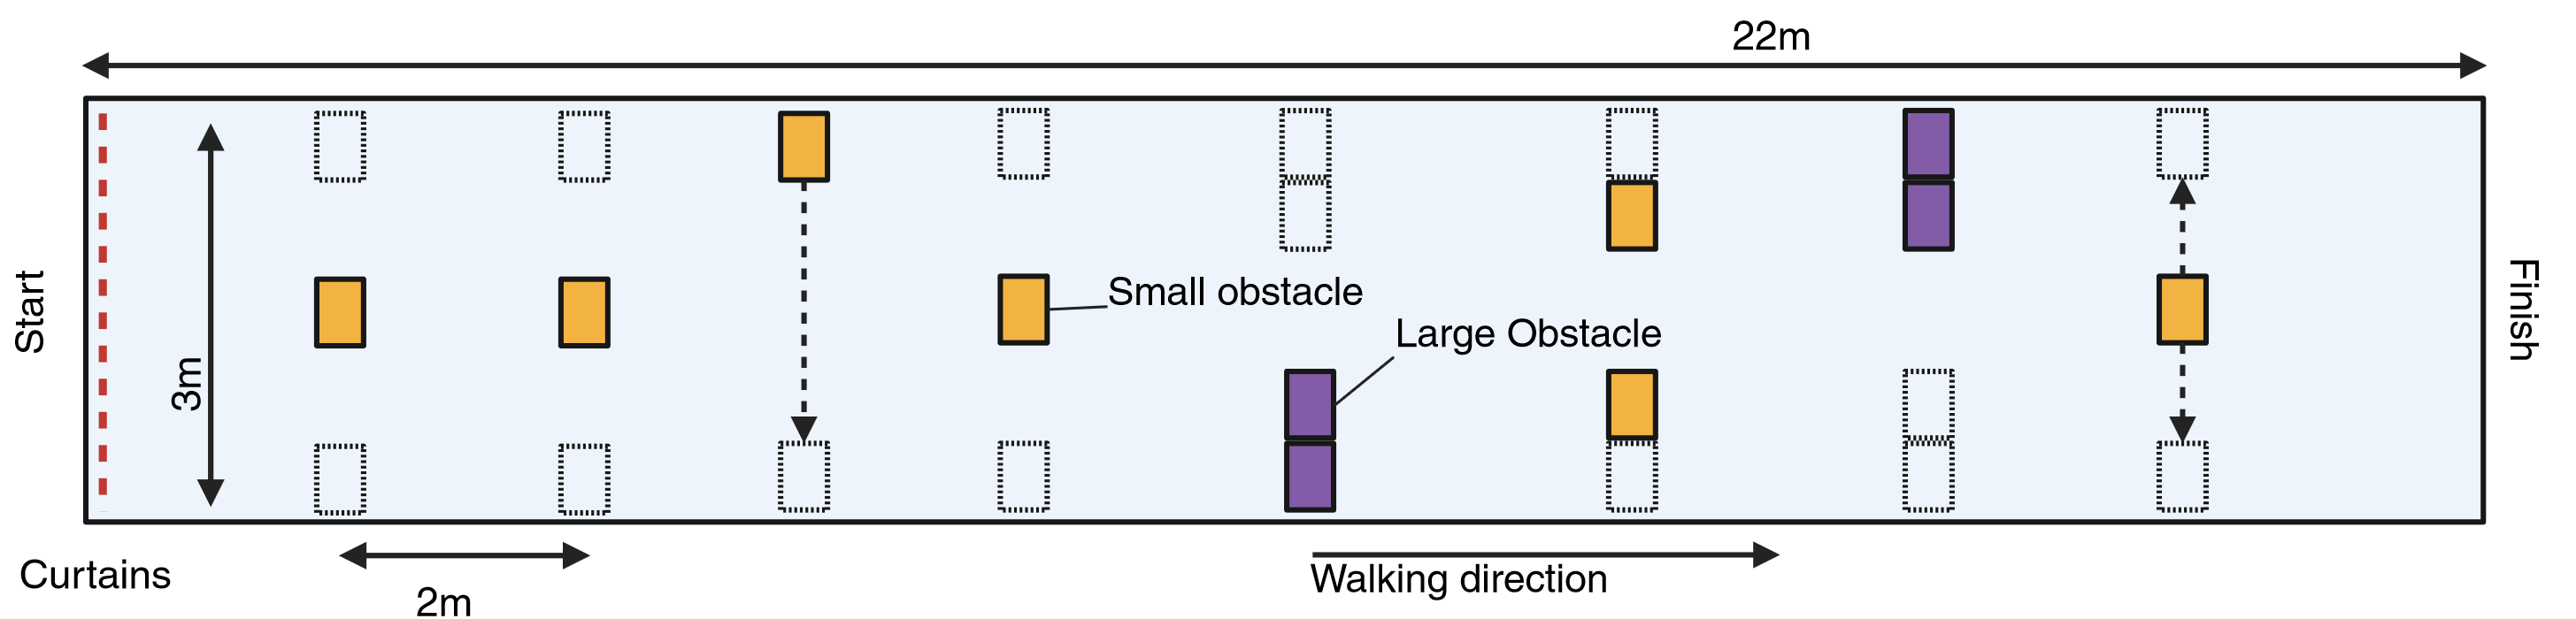
\includegraphics[width=1.0\textwidth]{imgs/Obstacle_course.png}
  \caption{| Overview of dynamic obstacle course setup with similarities to the experimental
    setup in work by~\textcite{deruytervansteveninckRealworldIndoorMobility2022}
    which used static objects only. Purple boxes indicate larger obstacles,
    while the orange boxes indicate small objects. Dashed boxes show options for
    alternative obstacle routes for participants, allowing for varies
    difficulty. Dashed arrows indicate the positions of dynamically moving
    objects via wheels. A curtain is placed at the start so participants cannot
    see the course before beginning the experiments. Each obstacle could be
    modified with varied texture overlays and varied lighting conditions.}\label{fig:obstacle_course}
\end{figure*}

\subsubsection*{Phase 2: Advanced AI and Neurophysiological Studies}
The second phase of the research focuses on implementing and testing advanced AI
algorithms alongside conducting neurophysiological studies to assess their
impact on visual perception. This phase builds on the groundwork laid in Phase 1
by introducing more sophisticated AI models, including Convolutional Neural
Networks (CNNs), Generative Adversarial Networks (GANs), and Reinforcement
Learning (RL) algorithms, with an emphasis on integrating edge computing for
real-time
processing~\parencite{granleyAdaptingBrainLikeNeural2022,elnabawyPVGANGenerativeAdversarial2022}.
Different algorithms are required in this phase to address the complex and
varied nature of dynamic visual environments. CNNs are utilized for their
effectiveness in image processing, GANs for their capability in generating
realistic data and enhancing image quality, and RL for its adaptive learning
abilities in real-time decision-making.

In Phase 2, the VR obstacle course will be designed to closely mimic real-world
environments, providing a more realistic and challenging setting for testing the
advanced AI algorithms. The VR course will feature a variety of obstacles,
including stationary and moving objects, to simulate dynamic environments.
Participants will navigate through different sections of the course, each
designed to test specific aspects of visual perception and navigation skills.
For instance, some sections will focus on object recognition and avoidance,
while others will test the participants' ability to navigate through cluttered
spaces. The VR setup will allow for the precise control and manipulation of the
environment, enabling the introduction of dynamic elements such as changing
lighting conditions and moving obstacles. This controlled variability is crucial
for evaluating the adaptability and robustness of the AI algorithms. Throughout
these trials, performance metrics such as navigation accuracy, speed, and
collision rates will be recorded, along with neurophysiological data to assess
the impact of the adaptive systems on visual perception. The obstacle course
will be modified based on the feedback and performance of the participants and
can be seen in Figure~\ref{fig:obstacle_course}.

The neurophysiological component of this phase will utilize (non-invasive)
Visual Evoked Potentials (VEP) and functional near-infrared spectroscopy (fNIRS)
to study the effects of the adaptive systems on visual
perception~\parencite{martinez-cagigalBrainComputerInterfaces2021,klistornerAnalysisMultifocalVisual2022,chenNeuralCorrelatesObstacle2017}.
These devices can be utilized in combination with the VR-setup. VEP data
includes response latency and amplitude of VEPs, spatial distribution, frequency
response, as well as changes in VEP wave patterns (P100, response 100 ms
post-stimulus). The fNIRS data includes hemodynamic responses, which allow for
identification of spatial and temporal activation of the visual cortex. Both
types of data will be used to measure the brain's response to different visual
stimuli and adaptive algorithms, providing insights into the effectiveness and
efficiency of the AI models as well as insights into plasticity and adaptation.
Participants, including both control and vision-impaired groups, will engage in
tasks such as navigation, object recognition, and reading, with performance
metrics including accuracy, response time, error rate, and trial duration, in
addition to neurophysiological data. By correlating these metrics with
neurophysiological responses, this phase aims to provide a deeper understanding
of how advanced AI-driven systems influence visual processing, thereby guiding
further refinements and improvements.

\subsubsection*{Justification of Phase 2}
Phase 2 is crucial for advancing the AI models developed in Phase 1 by testing
them in more complex and dynamic environments. This phase allows for the
exploration of the neurophysiological impacts of the AI-driven systems,
providing critical insights into how these systems interact with the human
visual system. The combination of advanced AI models and neurophysiological
assessments is necessary to ensure that the developed systems are not only
effective but also biologically plausible and beneficial for users.

\subsubsection*{Phase 3: Full-scale Experiments and Final Analysis}
The final phase of the research involves conducting extensive behavioral and
neurophysiological experiments with larger participant groups to validate the
effectiveness and reliability of the developed AI systems. This phase will
encompass a comprehensive set of behavioral experiments designed to collect
extensive performance data from a larger cohort, including control groups,
vision-impaired participants, and those with severe vision loss, thereby
enabling a robust evaluation of the system's efficacy in diverse real-world
scenarios. Concurrently, neurophysiological studies will continue with an
expanded participant group to ensure the generalizability of the findings.
Detailed analysis of patterns and insights derived from the collected data will
be performed to fine-tune the AI models and validate the improvements made
throughout the research. The ultimate aim of this phase is to ensure that the
AI-driven visual prosthetic system is ready for real-world application,
significantly enhancing the visual experiences of users with visual impairments
and contributing valuable knowledge to the field of neuroprosthetics.

\subsubsection*{Justification of Phase 3}
Phase 3 is essential for validating the developed AI systems on a larger scale
and in real-world scenarios. This phase aims to confirm the effectiveness and
reliability of the AI models by testing them with a more diverse and extensive
participant group. The comprehensive data collection and analysis will provide
robust evidence of the system's efficacy, ensuring that the AI-driven visual
prosthetic system is ready for practical deployment. Additionally, the
continuation of neurophysiological studies in this phase will ensure that the
improvements made are biologically grounded and beneficial across a broader
spectrum of users.

\subsection*{Risk Assessment and Feasibility}
Conducting this research involves several potential risks and challenges. These
include the technical difficulties of developing and integrating advanced AI
algorithms, the variability in neurophysiological responses among participants,
and the logistical complexities of managing VR-based experiments. To mitigate
these risks, the research will employ a phased approach, allowing for
incremental testing and refinement of the AI models. Additionally, the use of
well-established deep learning frameworks and neurophysiological measurement
techniques will enhance the reliability and validity of the findings. Ethical
considerations, including informed consent and the protection of participant
data, will be strictly adhered to throughout the study. The feasibility of the
research is supported by preliminary studies demonstrating the potential of AI
and VR in enhancing visual prosthetics, and by the availability of
state-of-the-art computational resources and expertise within the research team.

\section*{Innovation}\label{sec:innovation}
\subsection*{AI-Enhanced Visual Prostheses}
The proposed research is pioneering in its integration of advanced artificial intelligence (AI) and virtual reality (VR) to develop and enhance visual prostheses. This innovative approach leverages state-of-the-art deep learning algorithms, such as Convolutional Neural Networks (CNNs), Generative Adversarial Networks (GANs), and Reinforcement Learning (RL), to process complex visual inputs and generate simplified phosphene patterns that are interpretable and useful for users. By embedding these AI algorithms within a VR environment, the system can dynamically adapt to changes in the visual scene, thereby providing real-time scene simplification and improving the responsiveness of the prosthetic device. This integration is expected to significantly enhance the user experience, offering more accurate and detailed visual representations that are crucial for navigating dynamic and complex environments. The incorporation of multi-modal feedback, including haptic and auditory cues, further enhances the system's ability to provide comprehensive sensory information, thus creating a more immersive and effective visual aid.

\subsection*{Real-world Applications}
The potential real-world applications of this research are profound,
particularly in terms of improving the quality of life for individuals with
severe visual impairments. By enabling these individuals to perceive their
surroundings more clearly and respond more effectively to dynamic changes, the
developed system can facilitate greater independence and confidence in daily
activities. The anticipated improvements in scene simplification and
responsiveness are not only expected to enhance basic navigation and object
recognition but also to support more complex tasks such as reading and social
interactions. Beyond the immediate benefits to end-users, this research has
broader implications for the field of neuroprosthetics and adaptive technology.
It demonstrates the feasibility and advantages of integrating AI and VR to
create more sophisticated and adaptive prosthetic devices, setting a new
standard for future developments. Moreover, the insights gained from this
research could inform the design and implementation of other types of neural
interfaces, potentially leading to advancements in treating various neurological
conditions and enhancing sensory augmentation devices. This project stands at
the forefront of a transformative shift in how technology can be harnessed to
improve human capabilities and overall well-being.

\section*{Future Impact}\label{sec:impact}
\subsection*{Contribution to the Field}
This research is poised to make significant contributions to the field of visual
cortical prostheses by advancing the integration of artificial intelligence (AI)
and virtual reality (VR) systems in developing adaptive visual aids. The
innovative AI algorithms and real-time processing capabilities proposed in this
study are expected to enhance the functionality and usability of visual
prostheses, offering more accurate and dynamic visual representations for users.
These advancements will address current limitations in phosphene resolution and
scene simplification, potentially transforming how visual information is
processed and perceived by individuals with visual impairments. Moreover, the
successful implementation of these technological advancements could pave the way
for future research and development in related areas, such as the optimization
of other neural interfaces and sensory augmentation devices. The insights gained
from this study will provide a valuable foundation for further exploration into
AI-enhanced neuroprosthetics, encouraging ongoing innovation and improvement in
this critical field.

The integration of advanced AI models in visual prostheses represents a
significant intersection with the field of computer vision. By leveraging
techniques from computer vision, such as object recognition and scene
understanding, the AI algorithms can generate more coherent and detailed visual
representations for users. The use of feedback systems based on human behavior
is crucial in this context. By analyzing behavioral responses to visual stimuli,
the AI models can be iteratively improved to better align with the perceptual
and cognitive processes of users. Simultaneously, the development of these
protheses can provide valuable insights into the human visual system and how it
can adapt to digital augmentation.

Feedback systems like RL, enable real-time adjustments to the AI algorithms
based on user interactions and performance metrics. For example, if a user
consistently struggles with recognizing certain objects or navigating through
specific environments, the AI can adapt its processing strategies to enhance the
clarity and relevance of the visual information provided. This dynamic
adaptation is essential for creating a more intuitive and effective user
experience.

\subsection*{Call to Action}
The importance of continued interdisciplinary research cannot be overstated in
the quest to advance visual prosthesis technology. This proposal underscores the
need for collaboration between neuroscience, engineering, and AI to fully
realize the potential of these groundbreaking elements in cutting-edge
technological possibility. By fostering partnerships across these disciplines,
we can accelerate the development of more effective and sophisticated visual
aids, ultimately improving the quality of life for individuals with severe
visual impairments. We encourage researchers, practitioners, and stakeholders in
these fields to work together, share knowledge, and contribute to the collective
effort to enhance neuroprosthetic devices. The future of visual cortical
prostheses depends on our ability to integrate diverse expertise and innovate at
the intersection of these dynamic and rapidly evolving fields.
\clearpage
\section*{Timetable}\label{sec:timetable}
\begin{figure*}[ht!]
  \centering
  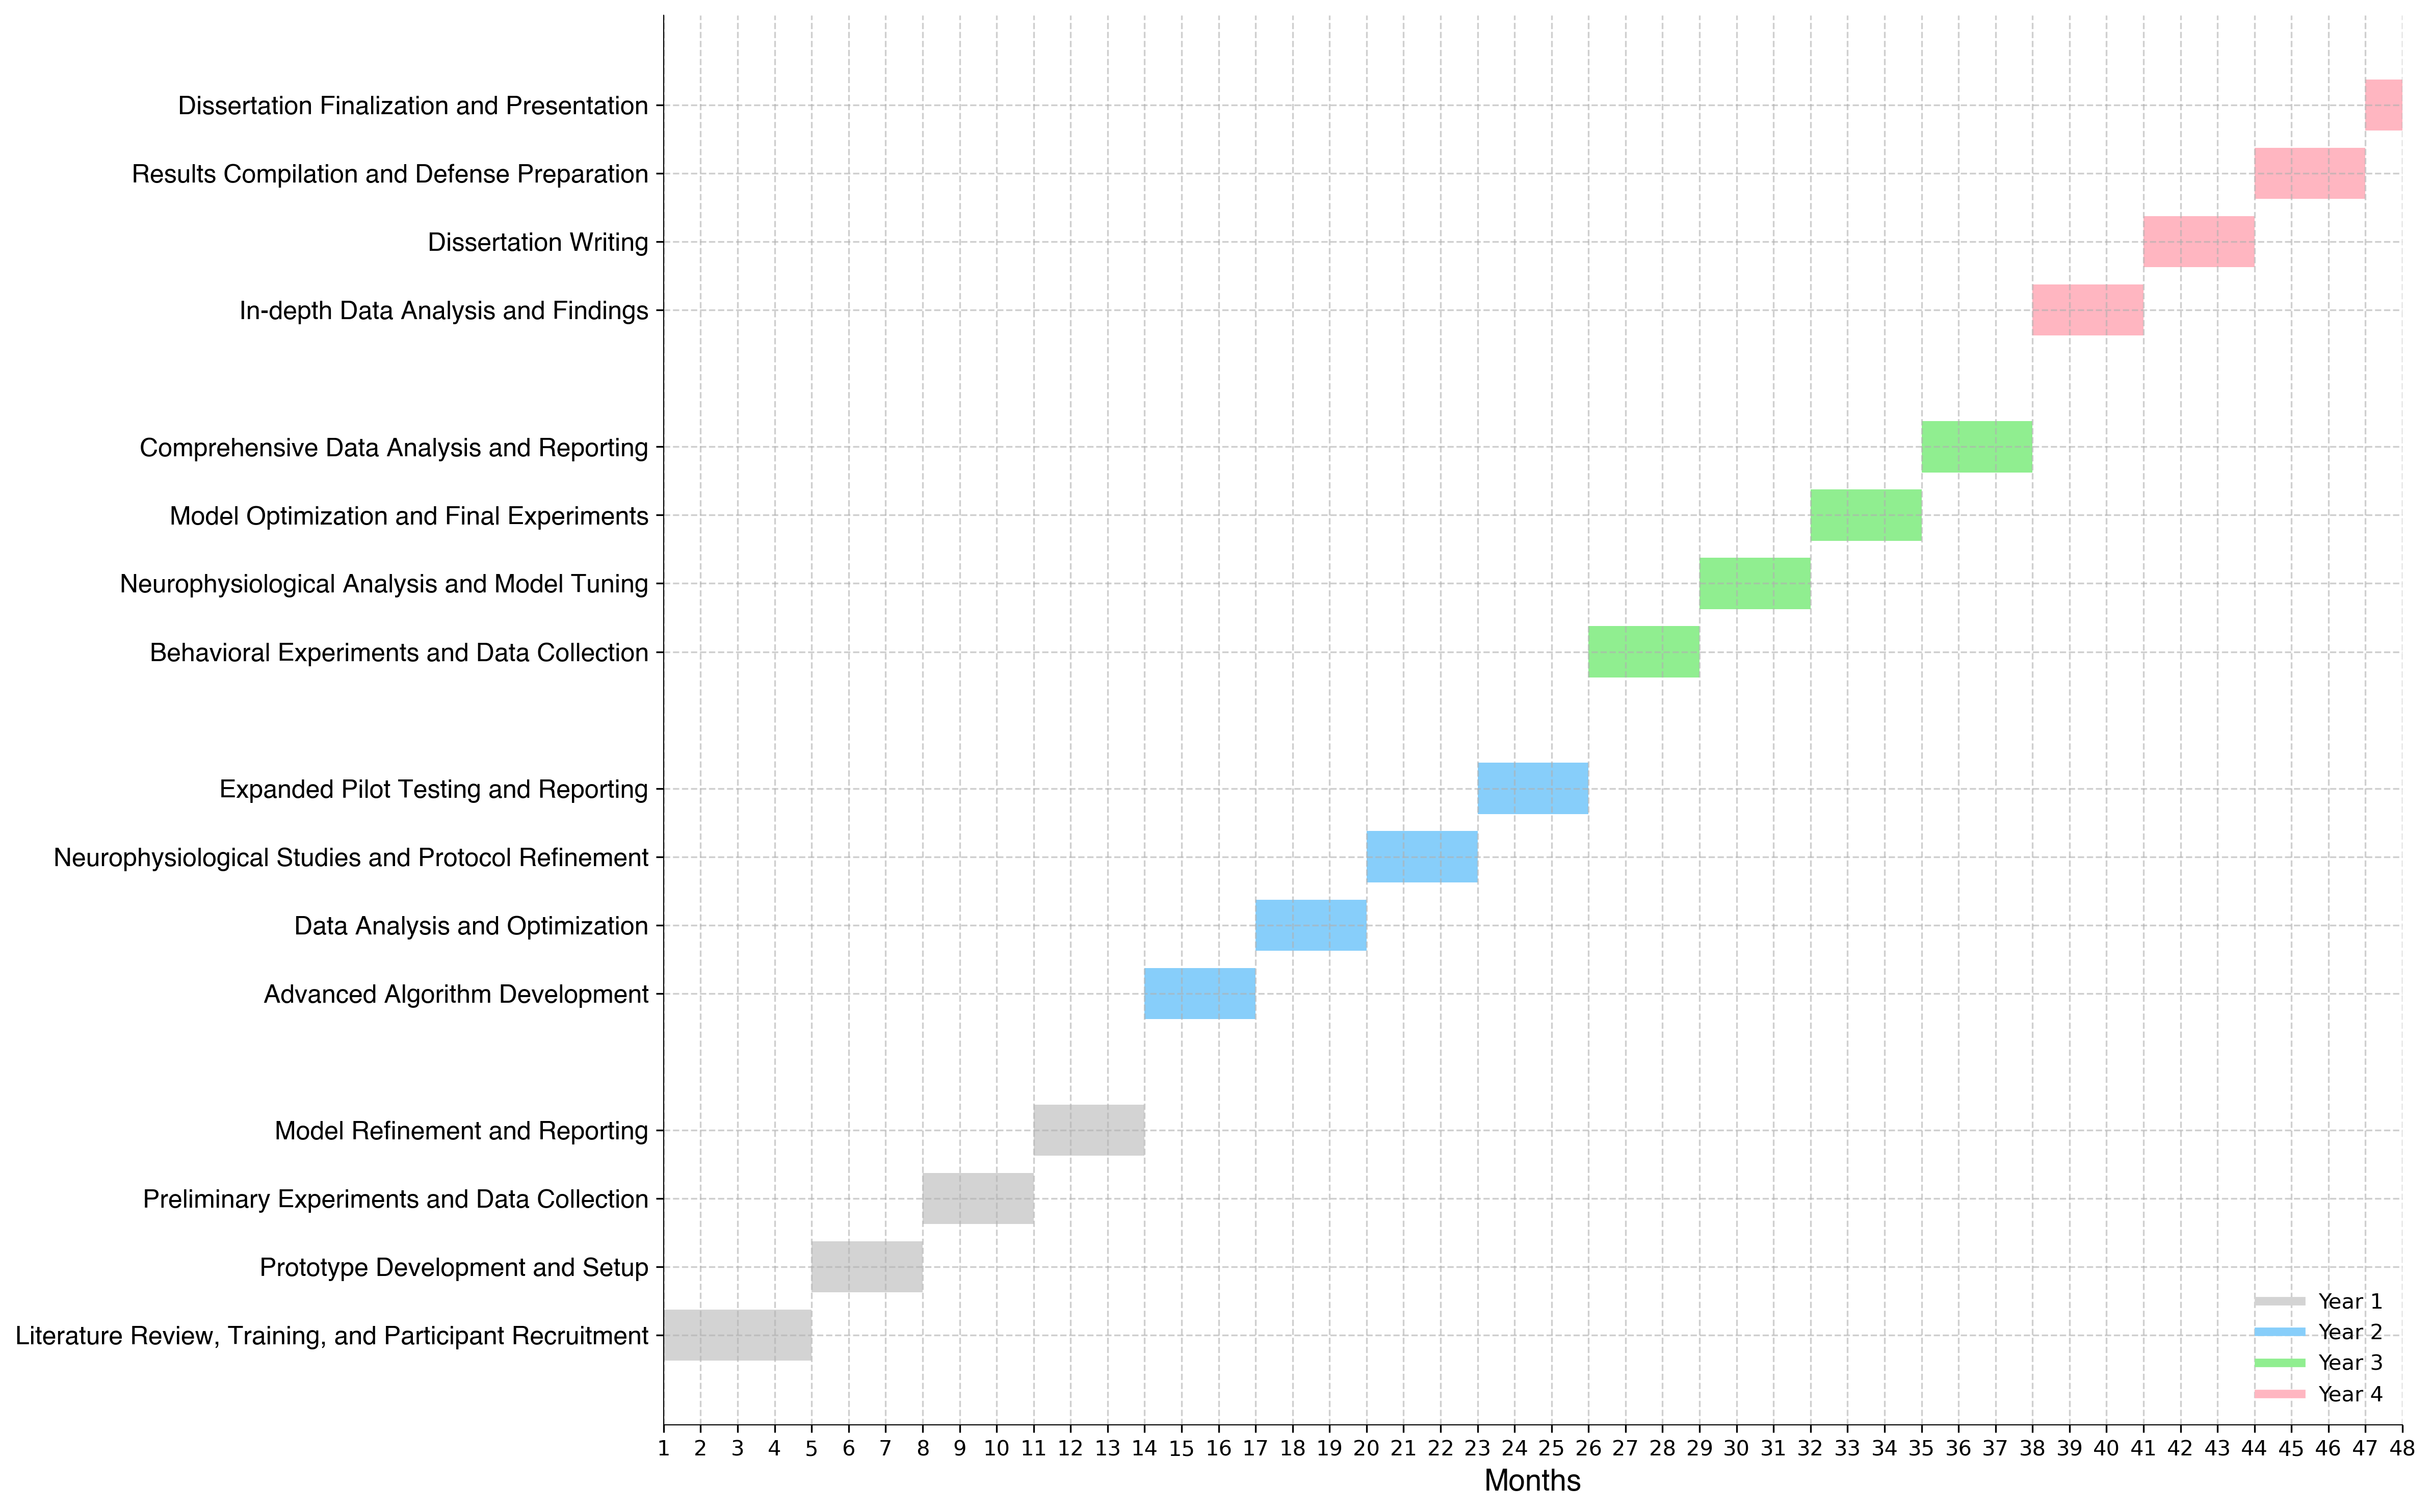
\includegraphics[width=1.0\textwidth]{imgs/Gannt_chart.png}
  \caption{| Gantt chart illustrating the timeline and key activities for a 4-year research project. The chart is divided into four distinct phases, one for each year. Each phase consists of various activities, which are represented by different colored bars indicating their start and duration in months. Year 1 focuses on preparation and initial research, Year 2 on advanced AI and pilot testing, Year 3 on full-scale experiments and data analysis, and Year 4 on final analysis and thesis writing. The color legend at the bottom right distinguishes between the years.}\label{fig:gannt_chart}
\end{figure*}
\pagebreak
\printbibliography%
\pagebreak
\section*{Rebuttal}\label{sec:rebuttal}
\noindent \textbf{Reviewer:} dr.\ F.\ Zeldenrust\\

\subsection*{General Comments}
\begin{itemize}
  \item Make the innovative aspects of the research more concrete in the summary, particularly focusing on improving the dynamic temporal aspects of phosphenes.\\
        \textcolor{blue}{\textit{Response: I have revised the summary to make the innovative aspects of the research more concrete, particularly focusing on improving the dynamic temporal aspects of phosphenes.}}

  \item On page 5, avoid starting the paragraph with ``However''. Instead, clearly reference the preceding issue.\\
        \textcolor{blue}{\textit{Response: I have revised the paragraph to clearly reference the preceding issue without starting with ``However''.}}

  \item In the introduction: Clearly delineate what is known, what is unknown, and what will be done to address the gap in knowledge.\\
        \textcolor{blue}{\textit{Response:  I have revised the introduction to clearly delineate what is known, what is unknown, and what will be done to address the gap in knowledge. The changes aim to enhance the clarity and focus of the introduction, making the research objectives more explicit.}}

  \item At the end of the introduction, reiterate the objectives of the research.\\
        \textcolor{blue}{\textit{Response: The objective of the proposed study
            is mentioned after the introduction in the section titled ``Research''
            and not at the end of the introduction to avoid redundancy.}}

  \item Reformulate the terms ``dynamic systems'' and ``visual aid systems''. Clarify that dynamic systems do not yet exist for such visual aid devices.\\
        \textcolor{blue}{\textit{Response: Changed the terminology to avoid confusion.}}

  \item Enhance the clarity of the reference when using ``simultaneously''.\\
        \textcolor{blue}{\textit{Response: Reformulated the sentences in the
            relevant paragraph to enhance clarity.}}

  \item Justify the necessity of Phase 1 and Phase 2, including the importance of training as preliminary work.\\
        \textcolor{blue}{\textit{Response: I have revised the ``Approach''
            section to justify the necessity of Phase 1, Phase 2 and Phase 3,
            emphasizing the importance of training and preliminary work. The changes
            highlight how each phase contributes to the overall research objectives
            and the foundational role of initial testing and training in ensuring
            the robustness and reliability of the AI models. It also explains why
            more extensive testing with larger participant groups is essential for validating the developed systems and preparing them for real-world applications.}}

  \item Elaborate on why different algorithms are required in Phase 2.\\
        \textcolor{blue}{\textit{Response:  I have elaborated on why different algorithms are required in Phase 2 within the text, highlighting the need to address the complex and varied nature of dynamic visual environments using CNNs, GANs, and RL\@. This addition emphasizes the complementary strengths of these algorithms in enhancing the overall system.}}

  \item Clarify how neurophysiological data will be utilized.\\
        \textcolor{blue}{\textit{Response: I have clarified how
            neurophysiological data will be utilized in the research for both types
            of data measurements, emphasizing
            their role in assessing the impact of the AI-driven systems on visual
            perception and guiding further refinements}}

  \item For Phase 1, focus on better deep learning implementation, and for Phase 2, describe the VR obstacle course.\\
        \textcolor{blue}{\textit{Response: I have revised the ``Approach'' section to focus on the better implementation of deep learning techniques in Phase 1 and provided a detailed description of the VR obstacle course used in Phase 2.}}

  \item Explain the transition between phases more clearly.\\
        \textcolor{blue}{\textit{Response: This has been done via the
            justification paragraphs for each phase.}}

  \item For Figure 2, provide a clearer explanation of its functionality and improve the reference link “adapted from”.\\
        \textcolor{blue}{\textit{Response: The figure caption has not been
            revised as both the caption and the inline text go over what is done for
            each block in the framework. The reference link has been updated to
            clarify that it is an adapted framework.}}

  \item Discuss the future impact and the relationship with computer vision, particularly how feedback systems based on human behavior can improve AI.\\
        \textcolor{blue}{\textit{Response: I have expanded the ``Future Impact'' section to discuss the relationship with computer vision and the role of feedback systems based on human behavior in improving AI.}}

  \item Add phases and year-end indications to the Gantt chart.\\
        \textcolor{blue}{\textit{Response: I changed the legend labels to phases
            as this was mistakenly labeled as years. I also added vertical lines
            to show the year cutoffs and increased the font size.}}

  \item Include a paragraph on risk assessment and feasibility.\\
        \textcolor{blue}{\textit{Response: I have included a paragraph on risk assessment and feasibility within the ``Approach'' section, following the description of the research phases. This addition addresses potential risks and challenges while highlighting the measures in place to ensure the feasibility and ethical conduct of the study.}}
\end{itemize}

\subsection*{Other Changes}
\begin{itemize}
  \item \textcolor{cyan}{\textit{Added a functional schematic representation of
            a visual cortical prosthesis in the ``Introduction'' section. I made this
            figure for my systematic review, but I think it makes the introduction more
            clear on how the visual percept is formed in context of the Simulated
            Phosphene Vision framework.}}
  \item \textcolor{green}{\textit{Final word count: 4997.}}
\end{itemize}

\subsection*{Final Remarks}
\begin{itemize}
  \item \textcolor{cyan}{\textit{After the presentation discussion it became clear that more
            attention could have given to the ``why'' of the research rather than the ``how''
            to make the need for the proposed plan more obvious. This is due to the
            complexity of how these AI systems could contribute to better prosthetics. A
            text that is written more in layman's terms would have been more beneficial.
            This is especially apparent in the summary and in the phasic approach where it
            is not abundantly clear why each phase is necessary. I will take this
            feedback into account for future research proposals. Lastly, it would have
            been nice to have added a proof of concept picture of the phosphene vision experience.}}
\end{itemize}

\end{document}